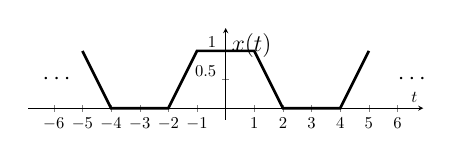
\begin{tikzpicture}[scale=0.6]
    \begin{axis}[
        x=.05\textwidth,y=0.1\textwidth,
    	axis y line=center,
    	axis x line=middle,
    	xlabel=$t$,ylabel={\Large $x(t)$},
    	xmin=-6.9,xmax=6.9,
    	ymin=-0.2,ymax=1.4,
    	xtick={-6,...,6},
    	xticklabel style = {xshift=0},
    	yticklabel style = {yshift=5}
	] 
	\addplot[
    	black,
    	ultra thick
    	] coordinates {
	(-5, 1) (-4, 0) (-2,0) (-1,1) (1,1) (2,0) (4,0) (5,1)
	} ;
	\node at (axis cs:6.5,0.5) {\Large $\cdots$} ;
	\node at (axis cs:-5.9,0.5) {\Large $\cdots$} ;
    \end{axis}
\end{tikzpicture}